\chapter{The extended Kalman filter}
\label{ch:ekf}

We now drop the compass. The state is the full pose $(p^x,p^y,\theta)$,
and both the motion model $f$ and the range--bearing model $h$ are
non-linear, so a Gaussian belief does not stay Gaussian. The \emph{extended}
Kalman filter keeps it Gaussian anyway: it replaces $f$ and $h$ by their
first-order Taylor expansions around the current estimate and then applies
the Kalman equations. This chapter derives the Jacobians, states the
filter, shows exactly what the linearisation throws away, and connects
the EKF update to Gauss--Newton optimisation.

\section{Linearisation}

The Kalman filter needs linear models. Near a given point every smooth
function looks linear: for a small deviation $\vect e$,
\[
  g(\vect a+\vect e)\approx g(\vect a)+G\,\vect e,\qquad
  G=\frac{\partial g}{\partial\x}(\vect a),\quad
  G_{ij}=\frac{\partial g_i}{\partial x_j}.
\]
The matrix $G$ is the \emph{Jacobian} of $g$ at $\vect a$: its column $j$
says how the output moves when the $j$-th input changes a little. In one
dimension it is the slope of the tangent (\cref{fig:linearisation}, left).
The EKF needs three Jacobians: $F$ and $V$ say how an error on the current
pose and an error on the control change the next pose, and $H$ says how an
error on the pose changes the measurement.

\begin{proposition}{Jacobians of the mower's models}{jacobians}
With $\theta'=\theta+\delta$, the motion model \eqref{eq:f} has
\[
  F=\frac{\partial f}{\partial\x}=\begin{pmatrix}1&0&-s\sin\theta'\\
  0&1&s\cos\theta'\\0&0&1\end{pmatrix},\qquad
  V=\frac{\partial f}{\partial\uu}=\begin{pmatrix}\cos\theta'&
  -s\sin\theta'\\\sin\theta'&s\cos\theta'\\0&1\end{pmatrix}.
\]
For a landmark at $\bell$, with $\vect{d}=\bell-\p$ and
$q=\norm{\vect{d}}^2$, the range--bearing model \eqref{eq:h} has
\[
  H=\frac{\partial h}{\partial\x}=\begin{pmatrix}-d_x/\sqrt q&-d_y/\sqrt q
  &0\\ d_y/q&-d_x/q&-1\end{pmatrix}.
\]
\end{proposition}

\begin{proof}
For $f$, differentiate component-wise; $\theta$ and $\delta$ enter only
through $\theta'$, whose derivative with respect to either is $1$. For the
range, $\nabla_{\p}\norm{\bell-\p}=-\vect{d}/\norm{\vect{d}}$. For the
bearing, $\partial\operatorname{atan2}(y,x)/\partial(x,y)=(-y,x)/
(x^2+y^2)$ and $\vect{d}$ depends on $\p$ with derivative $-I$, which
gives $(d_y,-d_x)/q$; the heading enters with coefficient $-1$. $\wrap$ is
locally a translation by a multiple of $2\pi$ and does not change
derivatives.
\end{proof}

Each entry can be read geometrically. The matrix $V$ is that of
\eqref{eq:firstorder}. The first two columns of $F$ say that a position
error is carried over unchanged. Its third column is the second column of
$V$: an error on the current heading acts exactly like a turn error, it
changes the new heading by the same amount and moves the mower sideways by
$s$ per radian (\cref{fig:tangent}). In $H$, the first row says that moving
towards the landmark shortens the range by the same amount, and that the
range does not depend on the heading. The second row says that moving
across the line of sight changes the bearing by the displacement divided
by the distance ($1/\sqrt q$ per unit), and that turning by an angle
changes the bearing by the opposite angle.

Hand-derived Jacobians are a classic source of bugs. The notebook and the
tests compare them with central finite differences; the largest
discrepancy is about $2\times10^{-9}$.

\section{The filter}

Suppose the belief is $\Normal(\hx,P)$, and write the true pose as
$\x_t=\hx+\vect e$ with $\vect e\sim\Normal(\vect0,P)$. Linearising $f$
around $(\hx,\uu)$ in both arguments,
\[
  \x_{t+1}=f(\hx+\vect e,\uu+\bepsilon)\approx f(\hx,\uu)+F\vect e
  +V\bepsilon .
\]
The right-hand side is an affine function of the independent Gaussians
$\vect e$ and $\bepsilon$, so by \cref{lem:affine} it is Gaussian with mean
$f(\hx,\uu)$ and covariance $FPF\T+VMV\T$: this is the prediction. In the
same way, around the predicted mean $\bx$,
\[
  \z=h(\x)+\vv\approx h(\bx)+H(\x-\bx)+\vv,
\]
a linear measurement of $\x$, up to the known constant $h(\bx)-H\bx$. The
Kalman update of \cref{thm:kf} then applies, with the innovation
$\z-h(\bx)$.

\begin{definition}{Extended Kalman filter}{ekf}
\begin{align*}
  &\textbf{predict:}&\bx&=f(\hx,\uu), & \bar P&=FPF\T+VMV\T,\\
  &\textbf{update:}& \y&=\z-h(\bx)\ \ (\text{bearings wrapped}), &
  S&=H\bar PH\T+R,\\
  && K&=\bar PH\T S^{-1}, & \hx&=\bx+K\y\ \ (\theta\ \text{wrapped}),
\end{align*}
$P=(I-KH)\bar P(I-KH)\T+KRK\T$, with $F,V$ evaluated at $(\hx,\uu)$ and
$H$ at $\bx$. With several visible landmarks, the measurements and the
rows of $H$ are stacked, and $R$ is block diagonal, with one copy of $R_1$
per landmark ($R=I\otimes R_1$).
\end{definition}

The \emph{mean} goes through the true non-linear functions; only the
\emph{covariance} goes through their Jacobians. The process noise enters
through the control, so its state-space covariance is $VMV\T$, of rank
two (\cref{prop:firstorder}); $\bar P$ stays positive definite because
$FPF\T$ is ($F$ is invertible, its determinant being $1$).

\begin{inwords}
The EKF pretends that, over the region where the mower probably is, the
world is flat: $f$ and $h$ are well approximated by their tangent planes.
It then applies the exact Kalman update to that flat world. When the
uncertainty is small compared with the curvature of $f$ and $h$, this is
an excellent approximation; when it is not, the next section shows what
goes wrong.
\end{inwords}

\paragraph{Angles.} Forgetting to wrap the bearing innovation is the most
common EKF bug in localisation. If the predicted bearing is $3.10$ and the
measured one is $-3.12$, the raw innovation is $-6.22$ instead of $+0.063$
(\cref{lem:wrap}), and the update throws the mower across the lawn.

On the standard run with four landmarks always in view, the EKF's position
RMSE is $1.13$, well below the range noise $\sigma_r=5$ and the
$\approx5$ units of position uncertainty that a bearing error of
$0.05$\,rad produces at 100 units. Each error component stays inside its
own $\pm2\sigma$ band about $95\%$ of the time: the filter is accurate and
honest.

\section{What linearisation throws away}

The EKF takes the mean of $g(X)$ to be $g$ of the mean. This is exact for
a linear $g$ and wrong for a curved one: where $g$ bends downwards, the
values of $g$ on both sides of the mean are below the tangent, and the
average of $g(X)$ is below $g(\bmu)$. The next proposition measures the
gap. In it, $\nabla^2g_i$ is the \emph{Hessian} of $g_i$, the matrix of its
second derivatives, and $\tr$ is the trace, the sum of the diagonal
entries.

\begin{proposition}{Second-order mean of a non-linear map}{secondorder}
Let $X\sim\Normal(\bmu,\Sigma)$ and let $g$ be four times continuously
differentiable with bounded fourth derivatives. Then
\[
  \E[g_i(X)]=g_i(\bmu)+\tfrac12\tr\bigl(\nabla^2g_i(\bmu)\,\Sigma\bigr)
  +O(\norm{\Sigma}^{2}),
\]
for each component $g_i$. The linearised mean $g(\bmu)$ is therefore
biased by $\tfrac12\tr(\nabla^2g_i\Sigma)$, to first order in $\Sigma$.
\end{proposition}

\begin{proof}
Taylor's theorem around $\bmu$ with $\vect{e}=X-\bmu$:
$g_i(X)=g_i(\bmu)+\nabla g_i\T\vect{e}+\tfrac12\vect{e}\T\nabla^2g_i
\vect{e}+\tfrac16D^3g_i[\vect{e},\vect{e},\vect{e}]+\rho(\vect{e})$ with
$|\rho(\vect{e})|\le C\norm{\vect{e}}^4$. Take expectations:
$\E[\vect{e}]=\vect0$,
$\E[\vect{e}\T A\vect{e}]=\E[\tr(A\vect e\vect e\T)]=\tr(A\Sigma)$, the
cubic term has expectation zero because the odd moments of a centred
Gaussian vanish, and $\E|\rho(\vect{e})|\le C\,\E\norm{\vect{e}}^4=
O(\norm{\Sigma}^2)$.
\end{proof}

For the heading, $\nabla^2\cos=-\cos$, so $\E[\cos\theta]\approx
\cos\bar\theta\,(1-\sigma_\theta^2/2)$, the first-order expansion of the
exact $e^{-\sigma_\theta^2/2}\cos\bar\theta$ (Exercise~\ref{ex:ecos}).
\Cref{fig:linearisation} shows it in one dimension: with
$\theta\sim\Normal(0.5,0.8^2)$, the EKF puts the mean of $\cos\theta$ at
$0.88$, against a true mean of $0.64$.

\begin{figure}[ht]
\centering
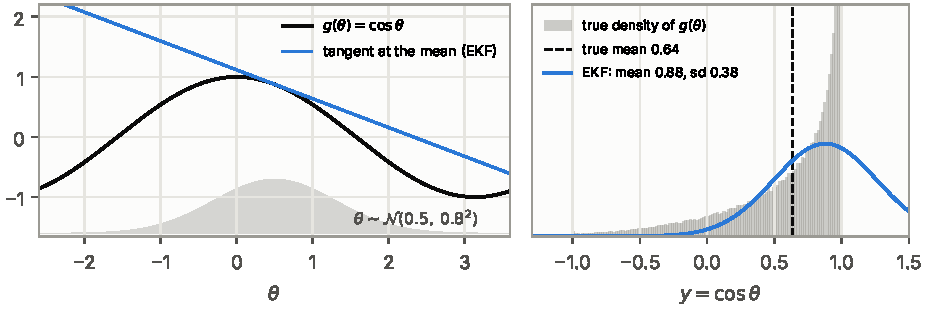
\includegraphics[width=\linewidth]{figures/ch04_linearisation.pdf}
\caption{Linearisation in one dimension. Left: $g(\theta)=\cos\theta$, the
input density (grey) and the tangent at its mean, which is all the EKF
uses. Right: the true density of $g(\theta)$ (histogram of $200\,000$
samples) and the EKF's Gaussian. The EKF's mean misses the curvature: it
is too high by $0.24$.}
\label{fig:linearisation}
\end{figure}

\Cref{fig:arc} shows the consequence. A mower known to within $1$ unit but
with a heading uncertainty of $\sigma_\theta=0.8$\,rad (about $45^\circ$)
drives 10 steps of 4 units straight ahead. The true distribution is an
arc. The EKF puts its mean at the tip of the arc, $11.05$ units ahead of
the true mean ($40(1-e^{-0.32})=10.95$ in theory), and its ellipse is a
needle, much too thin along the direction of travel.

\begin{figure}[ht]
\centering
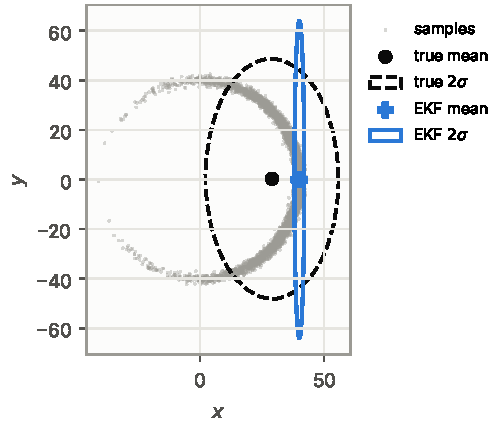
\includegraphics{figures/ch04_arc.pdf}
\caption{Forty units driven with a $45^\circ$ heading uncertainty. Grey:
5\,000 samples of the true distribution, with its mean and $2\sigma$
ellipse (dashed). Blue: the EKF's prediction, mean through $f$ and
covariance through $F$.}
\label{fig:arc}
\end{figure}

\section{Over-confidence}

Inside the filter, the same mechanism makes the EKF \emph{over-confident}
after an uncertain start. Twenty runs start from an estimate drawn from
$\Normal(\x_0,P_0)$ with $\sigma_{xy}=30$ and $\sigma_\theta=0.8$; the
sensor range is limited to 110 units, so that only one or two landmarks are
seen at a time. The average NEES (\cref{fig:ekftransient}) is $297$ after
the first update, $63$ after five and $6.5$ after twenty, against an
expected value of $3$.

\begin{figure}[ht]
\centering
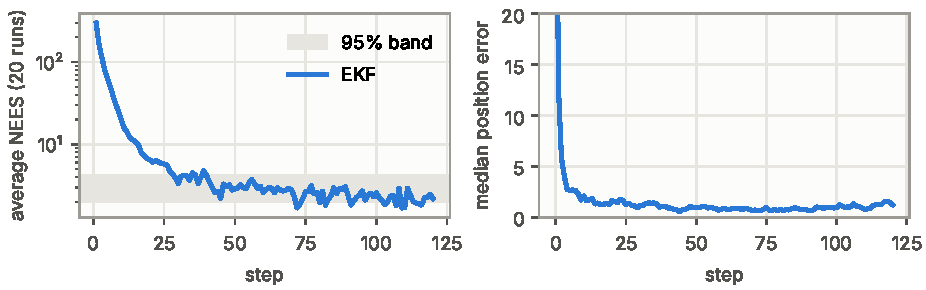
\includegraphics[width=\linewidth]{figures/ch04_transient.pdf}
\caption{EKF after an uncertain start (20 runs). Left: average NEES (log
scale) and the $95\%$ band for $n=3$. Right: median position error. The
filter converges, but for about twenty steps its covariance claims tens
to hundreds of times more precision than it has.}
\label{fig:ekftransient}
\end{figure}

The mechanism is easy to see. The Jacobian $H$ is evaluated at the
estimate $\bx$, which is tens of units and up to a radian away from the
truth. The update then treats the measurement as a linear function of the
state with \emph{that} slope, and $H\T R^{-1}H$ (\cref{prop:information})
adds information along directions computed at the wrong place. The
covariance shrinks as if the measurement had pinned the state down, while
the estimate has only moved part of the way. The next update, with a
small $\bar P$, then gives the new measurements little weight. If the error
had been larger, that false confidence could have made the filter reject
(by gating, \cref{sec:ekf-association}) the very measurements that would
have corrected it.

Common remedies: inflate $Q$ or $R$ while the uncertainty is large (cheap
and ad hoc); propagate the uncertainty without linearising (the UKF,
Chapter~\ref{ch:ukf}); or \emph{iterate} the update.

\section{The update as one Gauss--Newton step}

There is another way to look at the update. The posterior density is the
product of the predicted belief and the likelihood; its \emph{mode} is the
most probable pose. Maximising a product of Gaussian densities is the same
as minimising the sum of their exponents, a least-squares problem.
\emph{Gauss--Newton} is the standard method for non-linear least squares:
linearise the non-linear residual at the current point, solve the
resulting linear least-squares problem exactly, and repeat from the
solution.

\begin{proposition}{EKF and iterated EKF updates are Gauss--Newton steps}{gaussnewton}
The posterior mode of $\Normal(\x;\bx,\bar P)\,\Normal(\z;h(\x),R)$
minimises
\[
  J(\x)=\tfrac12\norm{\x-\bx}_{\bar P}^2+\tfrac12\norm{\z-h(\x)}_R^2,
  \qquad\norm{\vect{e}}_A^2=\vect{e}\T A^{-1}\vect{e}.
\]
One Gauss--Newton step on $J$ from $\x_i$, with $H_i=\partial h/\partial
\x(\x_i)$, gives
\begin{equation}\label{eq:iekf}
  \x_{i+1}=\bx+K_i\bigl(\z-h(\x_i)-H_i(\bx-\x_i)\bigr),\qquad
  K_i=\bar PH_i\T(H_i\bar PH_i\T+R)^{-1}.
\end{equation}
From $\x_0=\bx$, the first step is exactly the EKF update. Iterating to
convergence is the \emph{iterated} EKF.
\end{proposition}

\begin{proof}
Gauss--Newton linearises the residual $\z-h(\x)\approx\z-h(\x_i)-H_i
(\x-\x_i)$ and minimises the resulting quadratic. Its minimiser satisfies
$(\bar P^{-1}+H_i\T R^{-1}H_i)(\x-\bx)=H_i\T R^{-1}(\z-h(\x_i)-H_i(\bx-
\x_i))$, obtained by setting the gradient to zero. By
\cref{prop:information} the inverse of the left matrix is
$P_i=(I-K_iH_i)\bar P$ and $P_iH_i\T R^{-1}=K_i$, which gives
\eqref{eq:iekf}. With $\x_0=\bx$ the bracket is $\z-h(\bx)=\y$.
\end{proof}

\begin{inwords}
The EKF update is one step of an optimiser on the right cost function,
stopped after the first iteration. When the estimate is far from the
truth, one step is not enough; iterating, with re-linearisation at each
step, gets closer to the true posterior mode. This is also the bridge to
modern SLAM, which solves the same least-squares problem for a whole
trajectory at once (Chapter~\ref{ch:choosing}).
\end{inwords}

\section{Data association}
\label{sec:ekf-association}

So far the sensor has said which landmark it saw. When it does not, the
EKF must decide, before it can update, which landmark produced each
measurement $\z_k$. The standard choice is \emph{maximum-likelihood}
(nearest-neighbour) association: for each candidate $j$, compute the
innovation $\y_{kj}=\z_k-h_j(\bx)$ (bearing wrapped) and its covariance
$S_j=H_j\bar PH_j\T+R_1$, and choose
\[
  j^\star=\arg\min_j\;\y_{kj}\T S_j^{-1}\y_{kj}+\log\det S_j,
\]
the landmark under which the measurement is most likely. Indeed, if
landmark $j$ produced the measurement, the innovation is approximately
$\Normal(\vect0,S_j)$, and $-2\log\Normal(\y;\vect0,S)=\y\T S^{-1}\y+
\log\det S+\text{constant}$. The quantity $\y\T S^{-1}\y$ is the squared
\emph{Mahalanobis distance}: the size of the innovation counted in
standard deviations. For the right landmark and a consistent filter it
follows a $\chi^2_2$ distribution (this is the NIS of
\cref{ch:kalman}). A \emph{gate} therefore rejects the measurement when
even the best Mahalanobis distance exceeds a high quantile of $\chi^2_2$:
such a measurement is too surprising to come from any known landmark.

This works as long as the estimate is good. Once it is off by more than
about half the spacing between landmarks, the nearest landmark is the
wrong one. The update then pulls the estimate \emph{further} in the wrong
direction and shrinks its covariance, which makes the next wrong
association even more likely. In the showdown of
Chapter~\ref{ch:choosing}, an EKF with nearest-neighbour association loses
the mower in half of the uncertain starts and in six kidnappings out of
eight.

\begin{practice}[\nb{03\_extended\_kalman\_filter.ipynb}, \code{ekf.py}]
\code{motion\_jacobians} and \code{range\_bearing\_jacobian} implement
\cref{prop:jacobians}; \code{EKF} implements \cref{def:ekf} with the
Joseph update and \code{association="known"} or \code{"nearest"}. The
notebook checks the Jacobians by finite differences, plots the
$\pm2\sigma$ bands, and reproduces \cref{fig:arc,fig:ekftransient}.
\end{practice}

\begin{mower}
A mower is most uncertain when it matters most: after start-up, after a
long stretch without fixes (under a tree, along a wall), or after it has
been moved by hand. Those are exactly the moments when the EKF is
over-confident. A practical system watches the NIS of
\cref{ch:kalman}; when it leaves its band, the EKF is re-initialised from a
more robust estimator, for instance a particle filter or a GNSS fix.
\end{mower}

\section*{What to remember from this chapter}
\addcontentsline{toc}{section}{What to remember}

\begin{enumerate}[nosep]
  \item The EKF keeps a Gaussian belief on the full pose. The mean goes
    through the true models $f$ and $h$; the covariance goes through their
    Jacobians $F$, $V$ and $H$, evaluated at the current estimate.
  \item Linearisation ignores curvature. The mean of a curved function is
    not the function of the mean: the EKF's prediction is biased, by
    $\tfrac12\tr(\nabla^2g\,\Sigma)$ to leading order, and its covariance
    is too thin.
  \item When the uncertainty is small the EKF is accurate, honest and
    cheap. After a very uncertain start it is over-confident: the
    Jacobians are computed at the wrong place.
  \item The EKF update is one Gauss--Newton step on a least-squares cost;
    iterating it (the iterated EKF) gets closer to the posterior mode.
  \item With unidentified landmarks the EKF must choose one association
    per measurement. A wrong choice is reinforced by the update, and the
    filter can lose the mower for good.
\end{enumerate}

\FloatBarrier
\section*{Exercises}
\addcontentsline{toc}{section}{Exercises}

\begin{enumerate}[label=\textbf{4.\arabic*},ref=4.\arabic*]
\item\label{ex:ekfexact} Show that if $f$ and $h$ are affine, the EKF is
  exactly the Kalman filter.
\item\label{ex:cosvar} Let $\theta\sim\Normal(0,\sigma^2)$ and
  $y=\cos\theta$. What mean and variance does linearisation at $0$ give for
  $y$? Compute the true ones, and evaluate both for $\sigma=0.8$.
\item\label{ex:rangebias} Using \cref{prop:secondorder}, show that the mean
  of the range to a landmark is biased upwards by about
  $\sigma_\perp^2/(2r)$, where $\sigma_\perp^2$ is the position variance
  perpendicular to the line of sight. Why perpendicular?
\item\label{ex:gate} With a gate at the $99\%$ quantile of $\chi^2_2$,
  what fraction of correct measurements does a consistent EKF reject? And
  an EKF whose innovation covariance $S$ is ten times too small?
\end{enumerate}

\subsection*{Solutions}

\textbf{4.1.} If $f(\x,\uu)=F\x+B\uu+\vect{c}$, its Jacobian is $F$ and
the EKF predicted covariance is $FPF\T+Q$; if the noise enters through
the control as $f(\x,\uu+\bepsilon)$, it is affine in $\bepsilon$ too and
$VMV\T$ is the exact covariance of the noise term. The mean $f(\hx,\uu)$
is the exact mean by linearity. For an affine $h(\x)=H\x+\vect{c}$, the
innovation is $\z-H\bx-\vect{c}$ and the remaining formulas are those of
\cref{thm:kf}. Linearisation is exact for affine maps, so every step
coincides.

\textbf{4.2.} At $0$, $\cos'(0)=0$: linearisation gives
$y\approx1$, with mean $1$ and variance $0$. Exactly,
$\E[y]=e^{-\sigma^2/2}$ (Exercise~\ref{ex:ecos}) and
$\E[y^2]=\E[(1+\cos2\theta)/2]=(1+e^{-2\sigma^2})/2$, so
$\Var(y)=\tfrac12(1-e^{-\sigma^2})^2$. For $\sigma=0.8$: mean $0.726$
(not $1$) and standard deviation $0.334$ (not $0$). Linearising at a
stationary point loses \emph{all} the uncertainty; this is the needle of
\cref{fig:arc}.

\textbf{4.3.} For $r(\p)=\norm{\bell-\p}$, $\nabla r=-\hat{\vect{d}}$ and
$\nabla^2r=(I-\hat{\vect{d}}\hat{\vect{d}}\T)/r$ with
$\hat{\vect d}=\vect{d}/r$. So
$\tfrac12\tr(\nabla^2r\,\Sigma)=\tfrac1{2r}(\tr\Sigma-\hat{\vect{d}}\T
\Sigma\hat{\vect{d}})=\sigma_\perp^2/(2r)$. Moving along the line of sight
changes the range linearly (no curvature); moving perpendicular to it
always increases the range, by Pythagoras, so the errors do not average
out. The bias is small far from the landmark and large close to it.

\textbf{4.4.} For a consistent filter, the Mahalanobis distance of a
correct measurement is $\chi^2_2$, whose $99\%$ quantile is
$-2\log0.01=9.21$; $1\%$ of correct measurements are rejected. If $S$ is
ten times too small, the actual distance is ten times the
$\chi^2_2$ variable, and it exceeds $9.21$ with probability
$e^{-0.921/2}=0.63$: the filter rejects most of the measurements that
would correct it.
